\documentclass{article}

\usepackage[utf8]{inputenc}
\usepackage{caption}
\usepackage{csquotes}
\usepackage{multicol}
\usepackage{enumerate}
\usepackage{float}
\usepackage{graphicx}
\usepackage{makecell}
\usepackage{mathtools}
\usepackage{pgfplots}
\usepackage{subcaption}
\usepackage{tikz}
\usepackage[a4paper, total={6in, 8in}]{geometry}

% Remove References from BibTeX heading
\usepackage{etoolbox}
\patchcmd{\thebibliography}{\section*{\refname}}{}{}{}

% Path for images
\graphicspath{ {./images/} }

% Make table headings bold
\renewcommand\theadfont{}
\renewcommand\theadalign{bc}

% Remove indentation
\setlength\parindent{0pt}

\setlength{\belowcaptionskip}{-4pt}


\title{
    Parameterising Simulated Annealing \\
    \large for the Travelling Salesman Problem
}

\author{
    Gary Sun \\
    \large University of New South Wales
}

\date{Nov 2021}

\begin{document}

% Reduce margin to squeeze everything in
\newgeometry{total={6in, 9in}}

\maketitle
\begin{abstract}
    \centering
    In this paper, we explore the impact of different values of initial temperatures and cooling rates for Simulated Annealing.
    These values are benchmarked using the Travelling Salesman Problem, to determine their impact on optimality and runtime. 
    Finally, we determine if there is a correlation between the initial temperature and cooling rate with the input cities, and hence a way to parameterise the temperature and cooling rate.
\end{abstract}
\tableofcontents
\restoregeometry

%%%%%%%%%%%%%%%%%%%%%%%%%%%%%%%%%%%%%%%%%%%%%%%%%%%%%%%%%%%%%%%%%%%%%%%%%%%%%%%%
%%%%%%%%%%%%%%%%%%%%%%%%%%%%%%%%%%%%%%%%%%%%%%%%%%%%%%%%%%%%%%%%%%%%%%%%%%%%%%%%
\newpage
\section{Introduction}
\subsection{The Travelling Salesman Problem}
The travelling salesman is an example of an NP-hard combinatorial optimisation problem.

It goes as follows:
\begin{quote}
Given a weighted graph, starting at a vertex, find the minimal cost to travel to all the vertices of the graph once, before returning to the starting vertex.
\end{quote}

It has many applications, both in practice and theory, for example in logistics (determining an optimal route of least cost), job scheduling (determining the best way to schedule a series of jobs on a set of machines) and also benchmarking optimisation algorithms
\\

The specific purpose of this project is to explore the "Symmetric" Travelling Salesman Problem, the graph is undirected (the weight along a path / edge is the same regardless of direction).
Whilst this halves the number of solutions as compared to the asymmetric TSP, it still has a super-polynomial running time as the number of solutions for $n$ cities is $(n - 1)! / 2$.

\begin{figure}[h]
    \centering
    \begin{tabular}{ |c|c| } 
        \hline
        \thead{City Count} & \thead{Path Configurations} \\ 
        \hline
        3 & 1 \\
        \hline
        5 & 12 \\
        \hline
        10 & $1.81 \times 10^{4}$ \\ 
        \hline
        20 & $6.08 \times 10^{16}$ \\
        \hline
        30 & $4.42 \times 10^{30}$ \\
        \hline
    \end{tabular}
    \caption{Number of path configurations per number of cities}
\end{figure}

\subsection{Algorithms for the Travelling Salesman Problem}

Due to the difficult nature of solving the TSP, there are two main categories of algorithms.

\begin{itemize}
    \item Exact algorithms
    \item Approximate algorithms
\end{itemize}

Exact algorithms have the benefit that they can find the optimal solution.
For example, the current record for the largest TSP problem contained 85 900 cities and was solved using an ILP formulation \cite{cook12}.
However, they generally suffer from a longer runtime.
\\

On the other hand, approximate algorithms find a near-optimal, whilst running relatively quickly \cite{helsgaun98}.
Hence, in practice, if the optimal is not required, it is suitable to use an approximate algorithm.
An example of a common algorithm that can be applied for finding approximate solutions is SA (Simulated Annealing).
\\

Note TSP can be solved efficiently deterministically through cutting plane algorithms, and approximately through the Lin-Kernighan heuristic.
The goal of experimenting with SA is mostly out of curiosity and interest, however may reveal insights into the SA algorithm in general.

%%%%%%%%%%%%%%%%%%%%%%%%%%%%%%%%%%%%%%%%%%%%%%%%%%%%%%%%%%%%%%%%%%%%%%%%%%%%%%%%
%%%%%%%%%%%%%%%%%%%%%%%%%%%%%%%%%%%%%%%%%%%%%%%%%%%%%%%%%%%%%%%%%%%%%%%%%%%%%%%%
\newpage
\section{Simulated Annealing}
Simulated Annealing is a stochastic global search optimisation algorithm.
Whilst greedy searches may get stuck in a local minimum, Simulated Annealing aims to overcome this by probabilistically accepting worse options, and has a higher chance of finding the global minimum.

In the context of TSP, we start with a random solution, and then try different "similar" solutions.
We then choose to accept this new "similar" solution based off the SA algorithm, and continue this process, until we have not found better similar solutions.
\\

\subsection{Origin}
It is based on annealing in metallurgy, where the structure of the material changes randomly rapidly. when the temperature is high.
As a result, in the beginning, SA may choose a solution, even if does not lead to an improvement in the objective function.
\\

However, over time as the temperature drops and loses its internal energy, the structure settles into a more stable form.
Hence, as the temperature drops, the SA algorithm will with a higher probability discard solutions that do not improve the objective function and always choose those that improve the objective function.
\\

Finally, the resulting material structure reaches its absolute (global) minimum internal energy configuration.
Similarly, the SA algorithm will then find an approximate (or the) optimal solution for maximising the objective function.
\\

Note the temperature and cooling rate has to be carefully selected.
If the temperature cools too fast, then the process may get stuck at a local minimum. 
This is similar to what happens in a greedy method, where the search gets stuck in a local minimum.
Hence, the introduction of the temperature, and probabilistic acceptance of worse states allows for a higher chance of finding the global minimum.
\\

\subsection{Process}

\begin{enumerate}[Step 1:]
    \item Choose a suitable initial temperature $T_0$, cooling rate $r < 1$, a feasible solution $\mathbf{x}^{(0)}$, iteration counter $k = 0$, and the objective function $f$.
    \item Then select a neighbouring solution $\mathbf{x}^{(k + 1)}$ to $\mathbf{x^{(k)}}$, where $\mathbf{x}^{(k)}$ is the current solution at iteration $k$.
    \item Calculate  $\Delta f = f(\mathbf{x^{(k + 1)}}) - f(\mathbf{x^{(k)}})$. We then choose to take $\mathbf{x}^{(k + 1)}$ as the new solution with the following probability $P(\Delta f)$
    $$ P(\Delta f) = 
    \begin{dcases*}
        1 & if $\Delta f > 0$, \\
        \exp {\left( \frac{\Delta f}{T_k} \right)} & else
    \end{dcases*}
    $$
    \item If we have reached the max iterations, then stop.
    \item Else, set $k = k + 1$, and $T_k = r T_k$, then go to Step 2.
\end{enumerate}

\subsection{Cooling Rate and Temperature}

The initial temperature of the system determines how likely it is to accept worse solutions.
As shown in the selection function $\exp(\frac{\Delta f}{T})$ the temperature of the system should be proportional to the possible loss.
Hence, \textbf{the temperature should be proportional to the values of the loss function} to retain the same probability of choosing a worse configuration.
Typically a temperature is chosen that will result in an acceptance ratio of 0.8 \cite{initial-temperature}.

\begin{figure}[H]
    \centering
    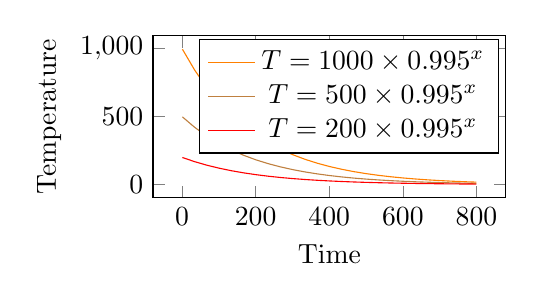
\begin{tikzpicture}
        \begin{axis}[
            width=0.5\textwidth,
            height=0.3\textwidth,
            xlabel=Time,
            ylabel=Temperature,
        ]
        \addplot[
            color=orange,
            domain=1:800
        ]
        {1000 * 0.995^x};
        \addlegendentry{$T = 1000 \times 0.995^x$}
        \addplot[
            color=brown,
            domain=1:800
        ]
        {500 * 0.995^x};
        \addlegendentry{$T = 500 \times 0.995^x$}
        \addplot[
            color=red,
            domain=1:800
        ]
        {200 * 0.995^x};
        \addlegendentry{$T = 200 \times 0.995^x$}
        \end{axis}
    \end{tikzpicture}
    \caption{Comparison initial temperatures cooling over time}
\end{figure}


The cooling rate on the other hand determines the rate of change of the probability that we accept worse configurations.
There is research \cite{fixed-temperature} to suggest that a constant temperature can produce optimal more configurations than that with a cooling rate, however this has only been tested for problems with less than 150 cities.
\\

Whilst there are different cooling schedules, geometric cooling tends to perform well compared to other general methods \cite{cooling-schedule}.
This is due to high temperatures at the beginning allowing for more searching, whilst low temperatures later allow it to converge to a solution quickly.
\\

Taking inspiration from nature, ignoring other properties, denser materials cool slower.
If the TSP behaves like so, \textbf{the greater the number of cities, the slower the system should cool} as it is "denser" in the number of cities.
Furthermore, if the number of cities is greater, there may also more local minimums, which can be mitigated by slower cooling.

\begin{figure}[H]
    \centering
    \begin{subfigure}[b]{0.48\textwidth}
        \centering
        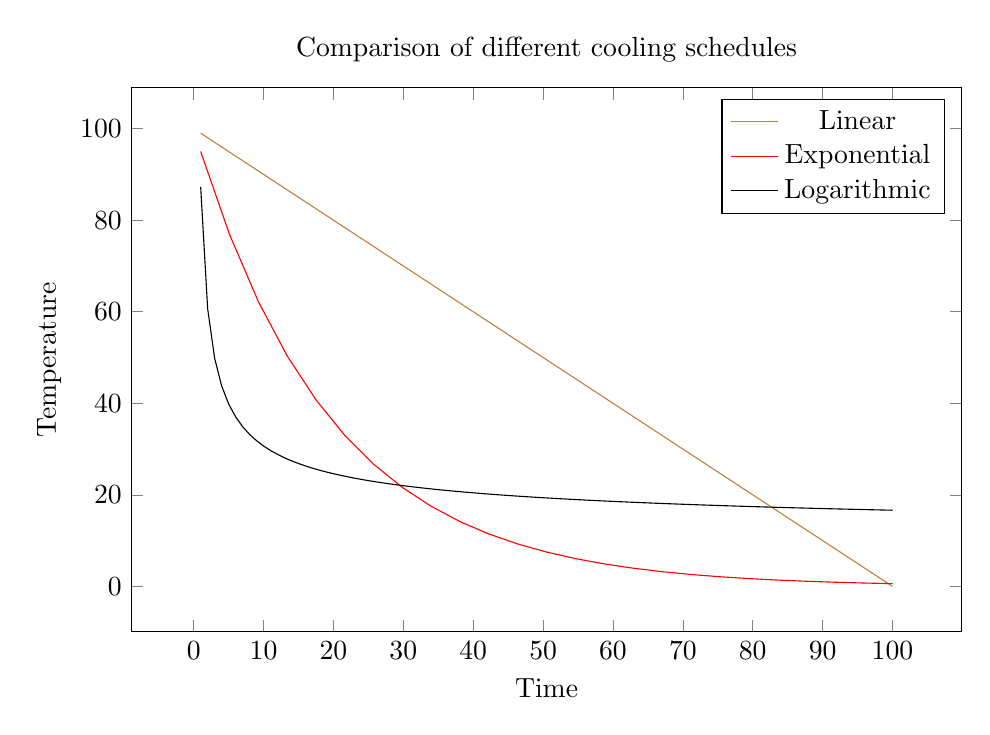
\begin{tikzpicture}
            \begin{axis}[
                title={Comparison of different cooling schedules},
                xlabel=Time,
                ylabel=Temperature,
                width=1\textwidth,
                height=0.7\textwidth,
            ]
            \addplot[
                color=brown,
                domain=1:100
            ]
            {100 - x};
            \addlegendentry{Linear}
            \addplot[
                color=red,
                domain=1:100
            ]
            {100 * 0.95^x};
            \addlegendentry{Exponential}
            \addplot[
                color=black,
                domain=1:100,
                samples=100
            ]
            {350/(1 + 10 * log10(1 + x))};
            \addlegendentry{Logarithmic}
            \end{axis}
        \end{tikzpicture}
    \end{subfigure}
    \hfill
    \begin{subfigure}[b]{0.48\textwidth}
        \centering
        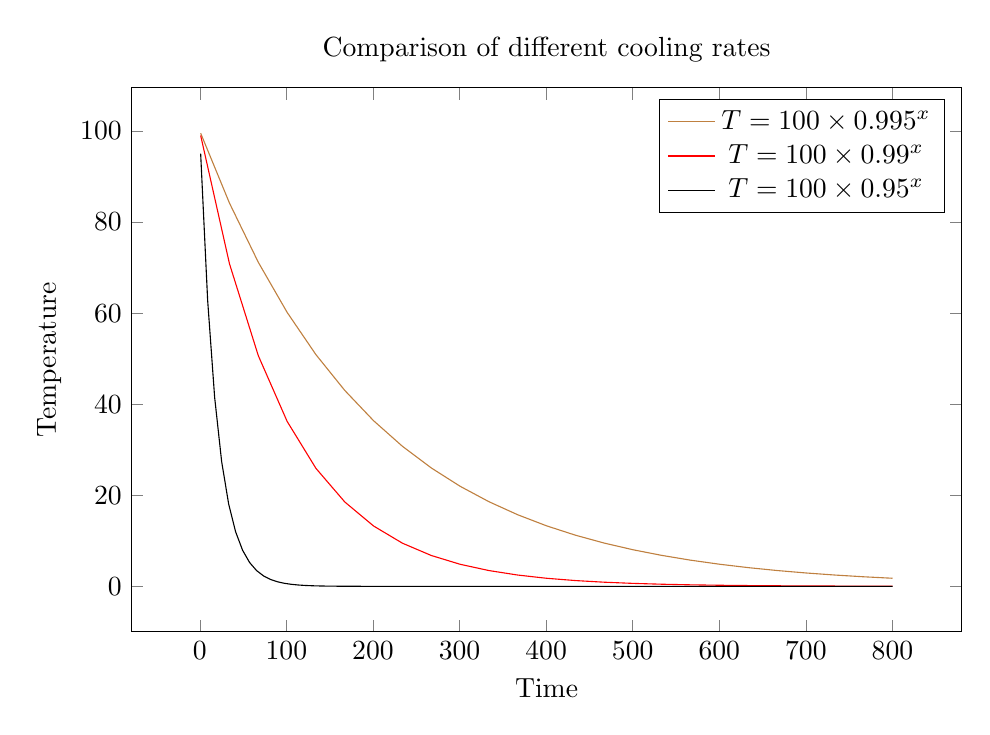
\begin{tikzpicture}
            \begin{axis}[
                title={Comparison of different cooling rates},
                xlabel=Time,
                ylabel=Temperature,
                width=1\textwidth,
                height=0.7\textwidth,
            ]
            \addplot[
                color=brown,
                domain=1:800
            ]
            {100 * 0.995^x};
            \addlegendentry{$T = 100 \times 0.995^x$}
            \addplot[
                color=red,
                domain=1:800
            ]
            {100 * 0.99^x};
            \addlegendentry{$T = 100 \times 0.99^x$}
            \addplot[
                color=black,
                domain=1:800,
                samples=100
            ]
            {100 * 0.95^x};
            \addlegendentry{$T = 100 \times 0.95^x$}
            \end{axis}
        \end{tikzpicture}
    \end{subfigure}
    \caption{Examples of different cooling schedules and rates where $r = 0.995$}
\end{figure}


%%%%%%%%%%%%%%%%%%%%%%%%%%%%%%%%%%%%%%%%%%%%%%%%%%%%%%%%%%%%%%%%%%%%%%%%%%%%%%%%
%%%%%%%%%%%%%%%%%%%%%%%%%%%%%%%%%%%%%%%%%%%%%%%%%%%%%%%%%%%%%%%%%%%%%%%%%%%%%%%%
\newpage
\section{Implementation}

\subsection{Controlled Variables}

\subsubsection{Objective Function}

Given a set of $n$ cities, where $c_{i,j}$ represents the cost of travelling between $i$ and $j$, we aim to find $O = \langle o_1, o_2, ..., o_n \rangle$ such that we 

$$\text{minimise}\left( \sum_{1 \leq i < n} c_{o_i, o_{i + 1}} + c_{n, 1}\right)$$

where $o_i = j$ means that city $j$ is in position $i$ of the path.
\\

\subsubsection{Selection Probability}

Although dependent on the temperature, the selection function penalises the selection of a local possible path configuration proportional to how much worse it is than the current path.

To do this, we use the Boltzmann Distribution as proposed by Metropolis \cite{metropolis},

$$p_i \propto \exp \left( \frac{- \epsilon_i}{kT} \right),$$

where
\begin{itemize}
    \item $p_i$ is the probability of choosing the state $i$,
    \item $\epsilon_i$ is the energy of the state (in our model, it is the cost of going from our state to the next)
    \item $k$ is Boltzmann's constant (ignored in our model)
    \item $T$ is the current temperature of the system
\end{itemize}


\begin{figure}[H]
    \centering
    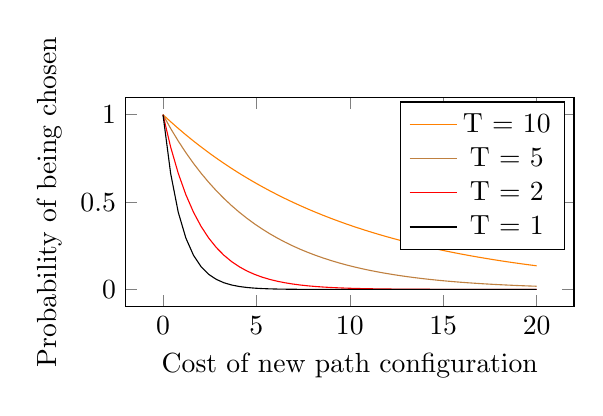
\begin{tikzpicture}
        \begin{axis}[
            width=0.6\textwidth,
            height=0.35\textwidth,
            xlabel=Cost of new path configuration,
            ylabel=Probability of being chosen
        ]
        \addplot[
            color=orange,
            domain=0:20,
            samples=50
        ]
        {exp(-x / 10)};
        \addlegendentry{T = 10}
        \addplot[
            color=brown,
            domain=0:20,
            samples=50
        ]
        {exp(-x / 5)};
        \addlegendentry{T = 5}
        \addplot[
            color=red,
            domain=0:20,
            samples=50
        ]
        {exp(-x / 2)};
        \addlegendentry{T = 2}
        \addplot[
            color=black,
            domain=0:20,
            samples=50
        ]
        {exp(-x / 1)};
        \addlegendentry{T = 1}
        \end{axis}
    \end{tikzpicture}
    \caption{Relationship between change in path cost and probability of selection}
\end{figure}

We can see that the greater the temperature, the higher the probability of choosing a worse configuration.
However, the greater the loss, the exponentially lower the probability of acceptance.
\\

\subsubsection{Local Search (2 opt)}

It is an important part of the algorithm to determine an algorithm to search for nearby possible solutions.
A well-known method is the \textbf{two-opt} method.
This involves selecting two random cities, re-orders the route between each other so that it does not.
\\

The example below shows before ($A \rightarrow B \rightarrow D \rightarrow C \rightarrow E \rightarrow F$) on the left, and after reversing the order between nodes B and E ($A \rightarrow B \rightarrow C \rightarrow D \rightarrow E \rightarrow F$) on the right.

\begin{figure}[!h]
    \centering
    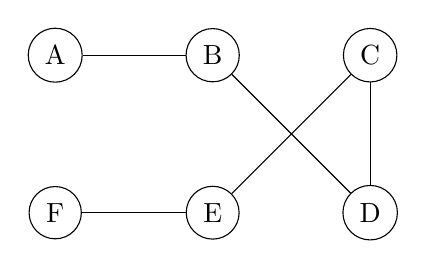
\begin{tikzpicture}
        \node[shape=circle,draw=black] (A) at (0,2) {A};
        \node[shape=circle,draw=black] (B) at (2,2) {B};
        \node[shape=circle,draw=black] (C) at (4,2) {C};
        \node[shape=circle,draw=black] (D) at (4,0) {D};
        \node[shape=circle,draw=black] (E) at (2,0) {E};
        \node[shape=circle,draw=black] (F) at (0,0) {F};
    
        \path [-](A) edge node[left] {} (B);
        \path [-](B) edge node[left] {} (D);
        \path [-](D) edge node[left] {} (C);
        \path [-](C) edge node[left] {} (E);
        \path [-](E) edge node[left] {} (F);
    \end{tikzpicture}
    \quad \quad \quad
    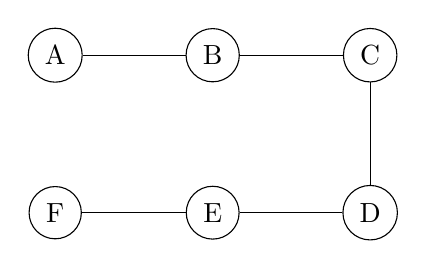
\begin{tikzpicture}
        \node[shape=circle,draw=black] (A) at (0,2) {A};
        \node[shape=circle,draw=black] (B) at (2,2) {B};
        \node[shape=circle,draw=black] (C) at (4,2) {C};
        \node[shape=circle,draw=black] (D) at (4,0) {D};
        \node[shape=circle,draw=black] (E) at (2,0) {E};
        \node[shape=circle,draw=black] (F) at (0,0) {F};
    
        \path [-](A) edge node[left] {} (B);
        \path [-](B) edge node[left] {} (C);
        \path [-](C) edge node[left] {} (D);
        \path [-](D) edge node[left] {} (E);
        \path [-](E) edge node[left] {} (F);
    \end{tikzpicture}
    \caption{two-opt between B and E}
\end{figure}

In the above scenario, the "before" distance will be shorter than the "after" distance if

$$\text{distance}(B, D) + \text{distance}(C, E) < \text{distance}(B, C) + \text{distance}(D, E)$$

which can be calculated in $O(1)$, whilst applying the two-opt runs in $O(n)$.
Hence, in the implementation, the loss of the new path configuration is calculated first before the path is changed.
Note that a more optimal method is the LKH (Lin–Kernighan heuristic), however, this is largely a variation of the two-opt and three-opt methods.
However, because of its difficulty in implementation \cite{helsgaun98}, and the main focus is on the temperature and cooling rate, only two-opt been implemented.

\subsubsection{Max Iterations}

There also has to be a way of determining when the solver has found what it considers the optimal solution.
The current implementations allows for the SA to continue iterating until it iterated \texttt{max\_iterations} times without finding a better solution.
From initial tests, it was possible for a slow cooling rate to have a very optimal solution before converging and then not find a better solution for many iterations.
Hence, the function to find a suitable \texttt{max\_iterations} gives a higher number of \texttt{max\_repeats} proportional to the cooling rate, and it is implemented as:

\begin{verbatim}
max_iterations = 10 // (1 - cooling_rate)
\end{verbatim}

\begin{figure}[H]
    \centering
    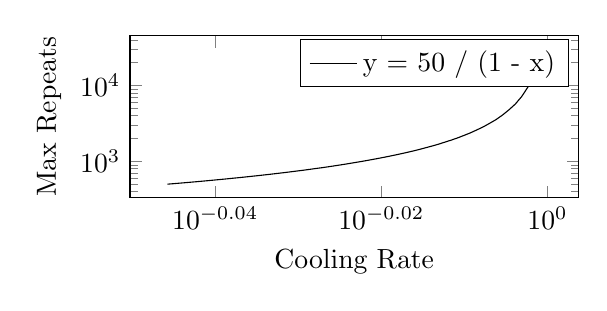
\begin{tikzpicture}
        \begin{axis}[
            width=0.6\textwidth,
            height=0.3\textwidth,
            xlabel=Cooling Rate,
            xmode=log,
            ylabel=Max Repeats,
            ymode=log,
        ]
        \addplot[
            color=black,
            domain=0.9:0.99999,
            samples=60
        ]
        {50 / (1 - x)};
        \addlegendentry{y = 50 / (1 - x)}
        \end{axis}
    \end{tikzpicture}
    \caption{Maximum repeats for each cooling rate}
\end{figure}

\subsection{Parameterisation}

We need to find a measure of the input that can correlate with the Cooling Rate and Temperature.

Ideally, these measures can be calculated quickly in polynomial time or better so that they can be found and then used to parameterise the Simulated Annealing algorithm before running it.

\subsubsection{Cooling Rate}

As the cooling rate allows for more exploration of nearby path configurations in the local search to prevent being stuck in a local minimum, we need a measure of "how likely it is to be stuck in a local minimum".

Whilst there may be other methods, the \textbf{number of cities will be used}, and finding it is as simple as the code below, which runs in $O(1)$ in python or at max $O(n)$ in a naive implementation.

\begin{verbatim}
def get_num_cities(cities: list[tuple[int, int]]) -> float:
    return len(cities)
\end{verbatim}

Hence, in the tests, different cooling rates will be tested on maps with different number of cities.
Their optimality and iteration count will then be compared to determine a suitable cooling rate based off the number of cities, where the other variables such as the average difference in distance of cities is the same.

\subsubsection{Temperature}

The temperature is relevant for determining the probability of accepting a worse configuration, as the loss from a worse configuration is divided by the temperature to find the probability.
As a result, the temperature needs to be high enough to accept worse configurations so that the search space is reduced, but not too high that the number of iterations is too great.
\\

Hence, it may be possible to parameterise the temperature with the average distance between cities.

However, initial tests showed zero better optimality from higher temperatures for higher city distances.
This is because it does not take into consideration the loss function: 
\\
Given the city coordinates \texttt{cities}, the ordering of the path \texttt{order} (where the first value is the first city to visit, and the second value the second city to visit, etc), return the change in total path length after applying two-opt between the city \texttt{a} and the city \texttt{b}.
This is implemented as:

\begin{verbatim}
from math import dist

def loss(cities: list[tuple[int, int]], order: list[int], a: int, b: int) -> float:
    n = len(cities)
    a1, a2 = cities[order[a]], cities[order[(a + 1) % n]]
    b1, b2 = cities[order[b]], cities[order[(b + 1) % n]]
    curr_dist = dist(a1, a2) + dist(b1, b2)
    swap_dist = dist(a1, b1) + dist(a2, b2)
    return swap_dist - curr_dist
\end{verbatim}

Hence, the return value of the \texttt{loss} function is proportional to the \textbf{difference in distances between the cities}.
\\

It has been suggested to take $T_0 = \Delta E_{\text{max}}$ where $\Delta E_{\text{max}}$ is the maximal cost difference in Kirkpatrick et al \cite{kirkpatrick}.
Another method described in Kirkpatrick et al \cite{kirkpatrick} is to choose $T_0$, and then perform a number of transitions, which will result in ratio of accepted probabilities $x_0$.
\\

A similar formula proposed by Johnson et al is to set the initial temperature $T_0 = \frac{\overline{\Delta E}}{\ln(X_0)}$ where $\overline{\Delta E}$ is an estimation of the cost of positive transitions.
Given that $X_0$ is often to be a value of around $0.8 - 0.9$, and $\ln(0.8)^{-1} \approx 5$, and $\ln(0.9) \approx 10$, the initial temperature may ideally be $\times 5$ to  $\times 10$ times larger than the average positive transition cost.
\\

Whilst, there are several methods to calculate the average positive transition cost \cite{initial-temperature}, they rely on samples from running SA multiple times.
The following code details how the average difference in distances (which is also the average positive transition cost) can be found in $O(n^2 \log n)$ using a dynamic programming (sliding window) approach:

\begin{verbatim}
from math import dist

def get_diff_city_dist(cities: list[tuple[int, int]]) -> float:
    n = len(cities)
    d = sorted([dist(cities[i], cities[j]) for i in range(n-1) for j in range(i+1,n)])
    m = len(d)
    
    prev_diff = sum([x - d[0] for x in d[1:]])
    total_diff = prev_diff
    for i in range(1, m):
        prev_diff = prev_diff - (d[i] - d[i - 1]) * (m - i)
        total_diff += prev_diff
    
    return total_diff / ((m * (m - 1)) / 2)
\end{verbatim}

Hence, in the tests, different temperatures will be tested on maps with different differences in the distances.
The maps will be generated with $n$ cities, and their positions scaled to adjust the distances.
Their optimality and iteration count will then be compared to determine a whether a suitable temperature based off the number of cities can be chosen.

\newpage
\subsection{Code}

The code is viewable online at https://github.com/angary/simulated-annealing-tsp.
\\

For the implementation there main code can be found in the \texttt{src/} folder, where the following files have the following purpose:

\begin{itemize}
    \item \texttt{src/solvers.py} 
    
    This contains classes that extend an abstract class \texttt{Solver} which contains abstract methods \texttt{get\_next\_order()} which runs one iteration of the solving algorithm, returning the current path it has found (used in the visualisation).
    It also contains the \texttt{SimulatedAnnealing} class, which takes in optional parameters \texttt{temperature} and \texttt{cooling\_rate}.
    
    \item \texttt{src/main.py} 
    
    This contains the code for running a visualisation of a problem from a file or randomly generated cities.
    It also has a method \texttt{solve()} which runs \texttt{get\_next\_order()} until the algorithm has determined that is has finished.
    
    \item \texttt{src/benchmark.py}
    
    This contains the code to benchmark the \texttt{SimulatedAnnealing} solver.
    It can either load in problems from a file or generate random problems (as detailed later in the report) and tests the \texttt{SimulatedAnnealing} solver with different options for \texttt{temperature} and \texttt{cooling\_rate}.
    The results are then stored in the \texttt{results/} folder.
    
    \item \texttt{src/setup.py}
    
    This contains the code for reading in the cities from a file in TSPLIB format.
    It also contains functions for determining the metrics such as average difference in city distances used for parameterising the Simulated Annealing algorithm.
    
    \item \texttt{src/config.py}
    
    This contains some configuration variables for both the visualisation and the testing.
    The testing variables are kept here to prevent import path issues when trying to access them from the Jupyter Notebooks.
    
\end{itemize}

The \texttt{data/} folder contains different problems taken from the TSPLIB library, where \texttt{.tsp} files contain problem instances, and \texttt{.opt.tour} files contain the optimal tour for the problem.
\\

The \texttt{report/} folder contains Jupyter Notebooks for visualising the results and also the source code for this report.

%%%%%%%%%%%%%%%%%%%%%%%%%%%%%%%%%%%%%%%%%%%%%%%%%%%%%%%%%%%%%%%%%%%%%%%%%%%%%%%%
%%%%%%%%%%%%%%%%%%%%%%%%%%%%%%%%%%%%%%%%%%%%%%%%%%%%%%%%%%%%%%%%%%%%%%%%%%%%%%%%
\newpage
\section{Experimentation}

\subsection{TSP Dataset Test}
First, the SA algorithm was benchmarked with TSPLIB \cite{tsplib} (a public library for TSP instances) with different initial temperatures and cooling rates.
The problems sets that were used are listed below

\begin{multicols}{6}
\begin{verbatim}
a280.tsp
att48.tsp
berlin52.tsp
ch130.tsp
ch150.tsp
gr666.tsp
pcb442.tsp
pr1002.tsp
pr2392.tsp
rd100.tsp
tsp225.tsp
ulysses22.tsp
\end{verbatim}
\end{multicols}

To conduct a test, the SA algorithm would be benchmarked, with a temperature and cooling rate of 0.
Then it would be run again with different combinations of temperature and cooling rates.
All of these tests would then be repeated multiple times as each run of SA can produce very different results.
The algorithm was then determined to have "finished" after it did not find a better solution after 1000 iterations.
\\

The following variables were used:

\begin{verbatim}
TEST_REPEATS = 20
TEMPERATURES = [10, 50, 100, 500, 1_000, 5_000]
COOLING_RATES = [0.999, 0.999_5, 0.999_9, 0.999_95]
\end{verbatim}

where \texttt{TEST\_REPEATS} is the number of times each test was repeated, \texttt{TEMPERATURE} is the initial temperature, and \texttt{COOLING\_RATE} is how much the temperature decreases each iteration.

\subsubsection{Results}

\begin{figure}[h]
    \centering
    \begin{tabular}{ |c|c|c|c| } 
        \hline
        \thead{Cooling Rate} & \thead{Mean Optimality \%} & \thead{Optimality Std Dev} & \thead{Mean Iterations} \\ 
        \hline
        0       & 0.7206 & 0.2151 & 69942 \\
        \hline
        0.999   & 0.7190 & 0.2151 & 71486 \\
        \hline
        0.9995  & 0.7214 & 0.2165 & 73394 \\ 
        \hline
        0.9999  & 0.7388 & 0.2263 & 94316 \\
        \hline
        0.99995 & 0.7549 & 0.2287 & 125381 \\
        \hline
    \end{tabular}
    \caption{Results of different cooling rates of the TSPLIB problems}
\end{figure}

\begin{figure}[h]
    \centering
    \begin{tabular}{ |c|c|c|c| } 
        \hline
        \thead{Temperature} & \thead{Mean Optimality \%} & \thead{Optimality Std Dev} & \thead{Mean Iterations} \\ 
        \hline
        0    & 0.7206 & 0.2151 & 69942 \\
        \hline
        10   & 0.7236 & 0.2171 & 74344 \\
        \hline
        50   & 0.7343 & 0.2207 & 81645 \\
        \hline
        100  & 0.7341 & 0.2230 & 84811 \\ 
        \hline
        500  & 0.7381 & 0.2233 & 95380 \\
        \hline
        1000 & 0.7367 & 0.2245 & 99195 \\
        \hline
        5000 & 0.7343 & 0.2245 & 111490 \\
        \hline
    \end{tabular}
    \caption{Results of different initial temperatures of the TSPLIB problems}
\end{figure}

\begin{figure}[h]
    \centering
    \begin{tabular}{ |c|c|c|c|c|c| } 
        \hline
        \thead{Name \\ } & \thead{City \\ Count} & \thead{Avg. City \\ Distance} & \thead{Avg. \\ Iterations} & \thead{Avg. \\ Optimality \%} & \thead{Optimality \\ Std. Dev. \%} \\
        \hline
        ulysses22.tsp & 22   & 4    & 84003  & 0.9991 & 0.0061 \\
        \hline
        att48.tsp     & 48   & 1608 & 17216  & 0.9576 & 0.0224 \\
        \hline
        berlin52.tsp  & 52   & 282  & 29205  & 0.9342 & 0.0359 \\ 
        \hline
        rd100.tsp     & 100  & 275  & 32775  & 0.8780 & 0.0446 \\
        \hline
        ch130.tsp     & 130  & 177  & 39815  & 0.8576 & 0.0437 \\
        \hline
        ch150.tsp     & 150  & 178  & 40381  & 0.8087 & 0.0470 \\
        \hline
        tsp225.tsp    & 225  & 91   & 56350  & 0.7502 & 0.0466 \\
        \hline
        a280.tsp      & 280  & 61   & 68501  & 0.6757 & 0.0424 \\
        \hline
        pcb442.tsp    & 442  & 872  & 78402  & 0.5924 & 0.0439 \\
        \hline
        gr666.tsp     & 666  & 44   & 133338 & 0.6904 & 0.0482 \\
        \hline
        pr1002.tsp    & 1002 & 3215 & 156407 & 0.4064 & 0.0295 \\
        \hline
        pr2392.tsp    & 2392 & 3186 & 347207 & 0.2458 & 0.019 \\
        \hline
    \end{tabular}
    \caption{Results of different TSPLIB problems}
\end{figure}

\begin{figure}[H]
\centering
    \begin{subfigure}{0.5\textwidth}
        \centering
        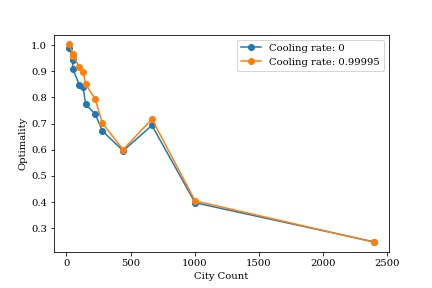
\includegraphics[width=0.95\linewidth]{images/tsplib_optimality_city_count.jpg}
        \caption{Cooling rate optimality for city count}
        \label{fig:sub1}
    \end{subfigure}%
    \begin{subfigure}{0.5\textwidth}
        \centering
        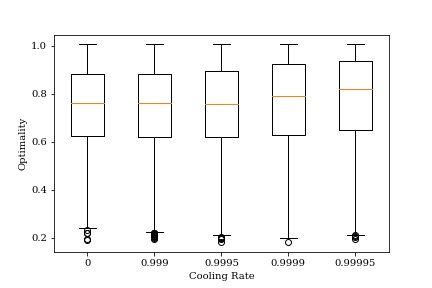
\includegraphics[width=0.95\linewidth]{images/tsplib_optimality_cooling_rate.jpg}
        \caption{Optimality for each cooling rate}
        \label{fig:sub2}
    \end{subfigure}
    \caption{Comparison between optimality, city counts, and cooling rate}
\end{figure}


\begin{figure}[H]
\centering
    \begin{subfigure}{0.5\textwidth}
        \centering
        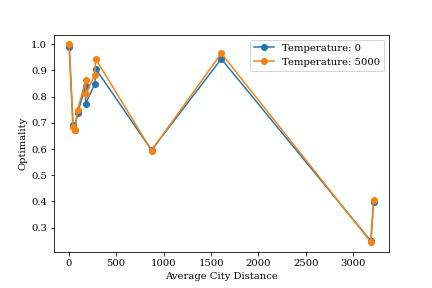
\includegraphics[width=0.95\linewidth]{images/tsplib_optimality_city_dist.jpg}
        \caption{Temp optimality for city distance}
        \label{fig:sub1}
    \end{subfigure}%
    \begin{subfigure}{0.5\textwidth}
        \centering  
        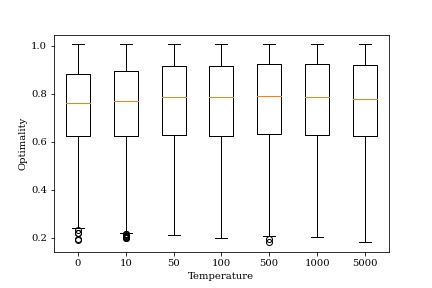
\includegraphics[width=0.95\linewidth]{images/tsplib_optimality_temperature.jpg}
        \caption{Optimality for each initial temperature}
        \label{fig:sub2}
    \end{subfigure}
    \caption{Comparison between optimality, city distances and temperatures}
\end{figure}

\subsubsection{Discussion}

From these results, there are a couple of observations that we can make
\begin{itemize}
    \item There is a negative exponential correlation between city count and temperature, however, there was a lack of correlation between city distance and optimality
    \item The higher the cooling rate, the better the optimality, however, there is no benefit to constantly increasing the temperature
    \item There was a logarithmic trend between cooling rate and iterations, and also a logarithmic trend between initial temperature and iterations
\end{itemize}

However, some issues need to be addressed
\begin{itemize}
    \item gr666.tsp is an outlier, is a dense cluster of cities, whilst the rest are sparsely scattered, resulting in higher average optimality as despite perhaps having a bad path configuration - because so many cities were close, the change in distance was small)
    \item since optimality has a very small correlation with optimality, we cannot tell if a certain temperature increases the optimality for an average city distance unless there is the same number of cities
\end{itemize}

To get more meaningful results, there needed to be a greater increase in the range of the cooling rate to determine the limit of a higher cooling rate.
The problem set used for the TSP problem also needs to be better controlled, as the impact of temperature on optimality for different temperatures could not be determined as optimality was more dependent on the number of cities.

\newpage
\subsection{Random Dataset Test}

Rather than experimenting with well known TSP problems such as those found in TSPLIB, the SA was tested using randomly generated cities.
The reasoning is that variables such as distances or city count can be controlled well whilst the other values are adjusted.
\\

As a result, specific maps could be generated for testing temperature (where the city count was kept the same, but differences in distance increased) and maps could be generated for testing cooling rate (where differences in distance was kept the same, but the city count was increased).
\\

To conduct the tests, the following variables were used:

\begin{verbatim}
MAP_COUNT = 4
TEST_REPEATS = 20
DIST_DIFFS = [1, 10, 100, 1_000, 10_000]
CITY_COUNTS = [10, 30, 100, 300, 1_000, 3_000]
CONST_CITY_COUNT = 400
CONST_DIST_DIFF = 20

TEMPERATURES = [0, 1, 10, 100, 1_000, 10_000]
COOLING_RATES = [0, 0.9, 0.99, 0.999, 0.999_9, 0.999_99]
CONST_TEMPERATURE = 40
CONST_COOLING_RATE = 0.9999
\end{verbatim}

where

\begin{itemize}
    \item \texttt{MAP\_COUNT} was the number of different generated maps for each test
    \item \texttt{TEST\_REPEATS} was how many times a test would be repeated with the same map, initial temperature and cooling rate
    \item \texttt{DIST\_DIFFS} is an array of the difference in distances between cities, used with \texttt{CONST\_CITY\_COUNT} to generate \texttt{MAP\_COUNT} maps for testing temperature
    \item \texttt{CITY\_COUNTS} is an array of the different number of cities, used with \texttt{CONST\_DIST\_DIFF} to generate \texttt{MAP\_COUNT} maps for testing cooling rate
    \item \texttt{TEMPERATURES} is an array of the different initial temperatures used, whilst \texttt{CONST\_COOLING\_RATE} was the cooling rate that was kept constant across the temperature tests
    \item \texttt{COOLING\_RATES} is an array of the different cooling rates used, whilst \texttt{CONST\_TEMPERATURE} was the temperature that was kept constant across the cooling rate tests
\end{itemize}

\newpage
\subsubsection{Results}

There was a very good trend between the a slower cooling rate and a more optimal solution, and more iterations.

\begin{figure}[H]
    \centering
    \begin{subfigure}{0.5\textwidth}
        \centering
        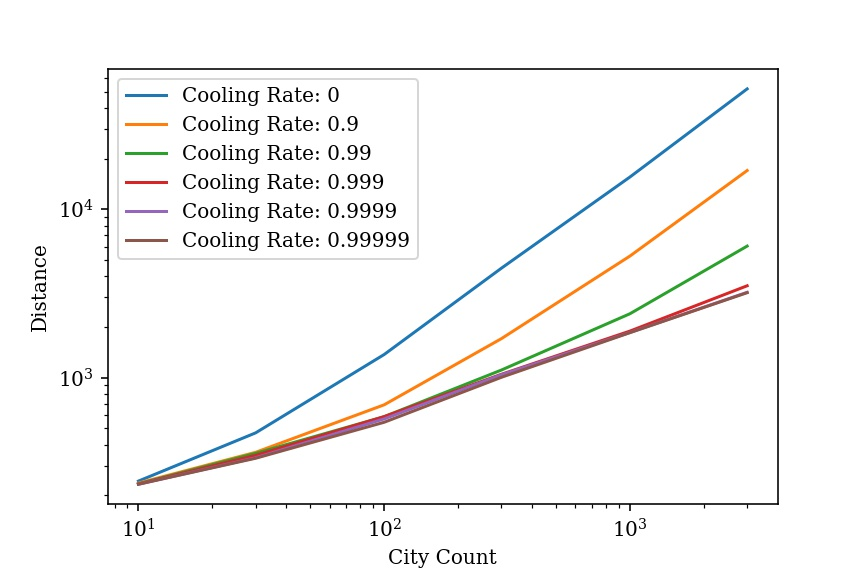
\includegraphics[width=1\linewidth]{images/rand_cooling_rate_city_count_distance.jpg}
        \caption{Absolute final distances}
        \label{fig:sub1}
    \end{subfigure}%
    \begin{subfigure}{0.5\textwidth}
        \centering
        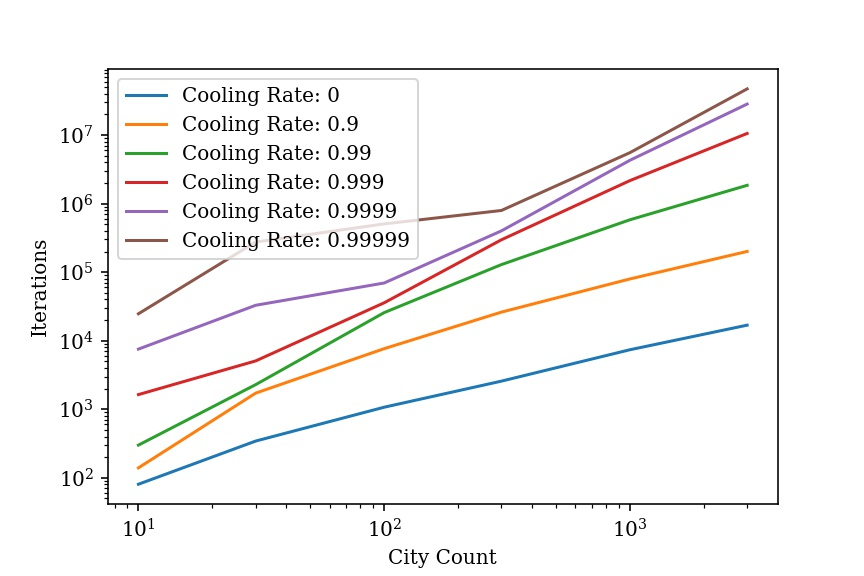
\includegraphics[width=1\linewidth]{images/rand_cooling_rate_city_count_iterations.jpg}
        \caption{Absolute iterations}
        \label{fig:sub2}
    \end{subfigure}
    \captionsetup{justification=centering}
    \label{rand-cooling-rate}
    \caption{Absolute comparison between final distances, and iterations, for different $r$}
\end{figure}

\begin{figure}[H]
    \centering
    \begin{subfigure}{0.5\textwidth}
        \centering
        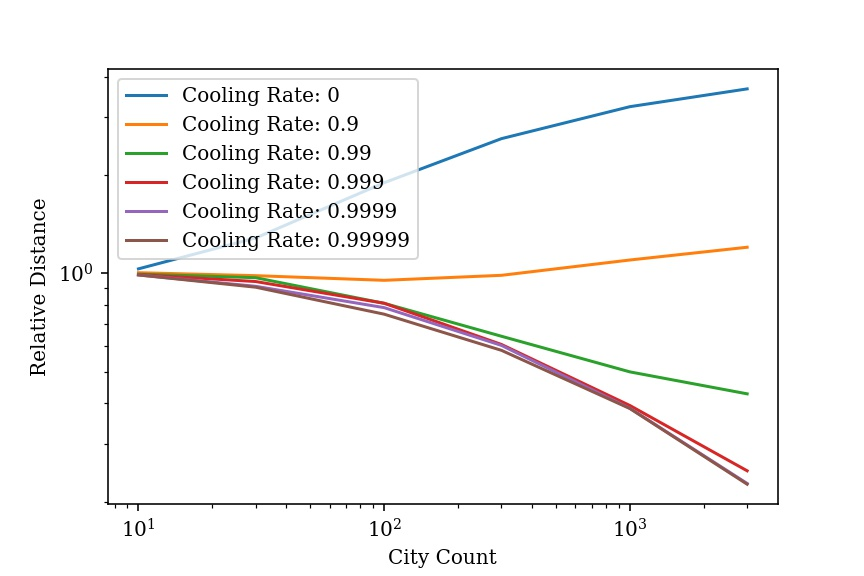
\includegraphics[width=1\linewidth]{images/rand_cooling_rate_city_count_distance_relative.jpg}
        \caption{Relative final distance}
        \label{fig:sub1}
    \end{subfigure}%
    \begin{subfigure}{0.5\textwidth}
        \centering
        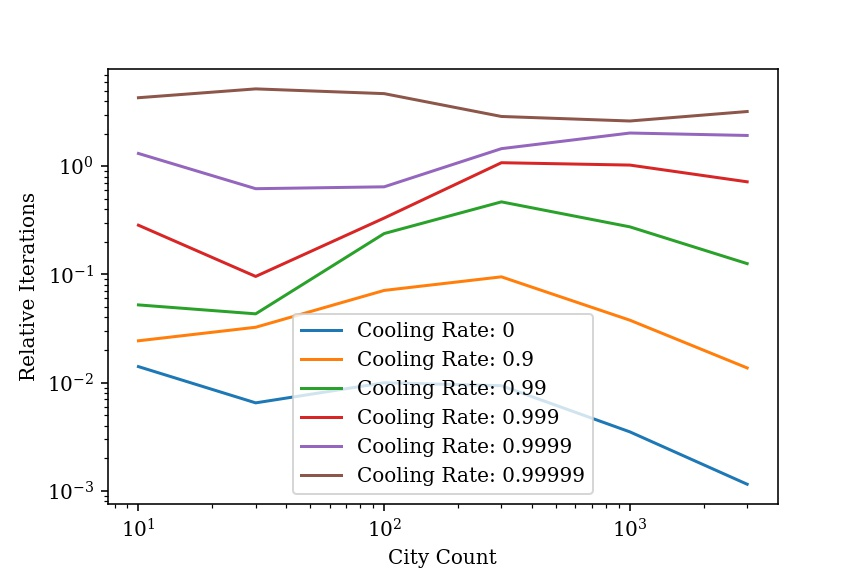
\includegraphics[width=1\linewidth]{images/rand_cooling_rate_city_count_iterations_relative.jpg}
        \caption{Relative iterations}
        \label{fig:sub2}
    \end{subfigure}
    \captionsetup{justification=centering}
    \label{rand-cooling-rate}
    \caption{Relative comparison between final distances, and iterations, for different $r$}
\end{figure}

An initial test was conducted for different $T_0$ and average difference in distances for $r = 0.995, n = 400$.
This resulted in little to no trend between the final distance.
Hence, another test was conducted where $r = 0.995, n = 800$.
\\

Both these tests resulted in negligible trends, and their results are shown below.

\begin{figure}[H]
    \centering
    \begin{subfigure}{0.45\textwidth}
        \centering
        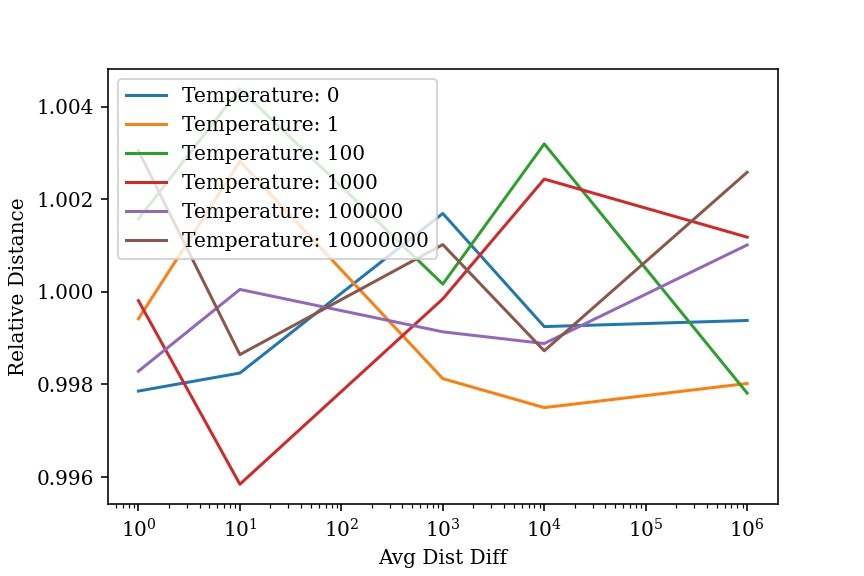
\includegraphics[width=1\linewidth]{images/rand_temperature_avg_dist_diff_distance_relative_400.jpg}
        \caption{Relative final distance, where $n = 400$}
    \end{subfigure}%
    \begin{subfigure}{0.45\textwidth}
        \centering
        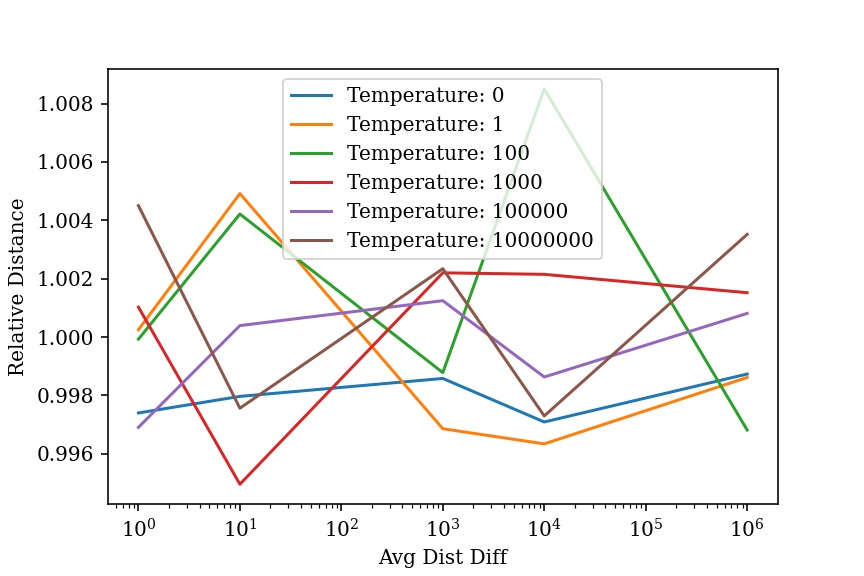
\includegraphics[width=1\linewidth]{images/rand_temperature_avg_dist_diff_distance_relative_800.jpg}
        \caption{Relative final distance, where $n = 800$}
    \end{subfigure}
    \captionsetup{justification=centering}
    \caption{Relative comparison between final distances, and iterations, for different $T_0$}
\end{figure}

The reasoning for this was assumed to be the fast cooling rate, meaning that the temperature cooled too fast towards a low level, essentially rendering the initial temperature irrelevant.
Hence, another test was conducted, where $r = 0.9999$, and $n = 400$.

\begin{figure}[H]
    \centering
    \begin{subfigure}{0.45\textwidth}
        \centering
        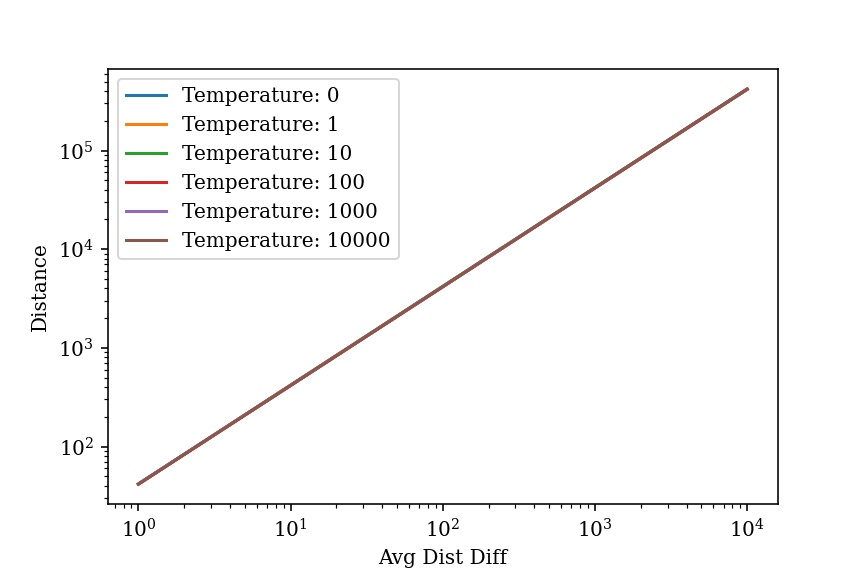
\includegraphics[width=1\linewidth]{images/rand_temperature_avg_dist_diff_distance.jpg}
        \caption{Final distance for different }
        \label{fig:sub1}
    \end{subfigure}%
    \begin{subfigure}{0.45\textwidth}
        \centering
        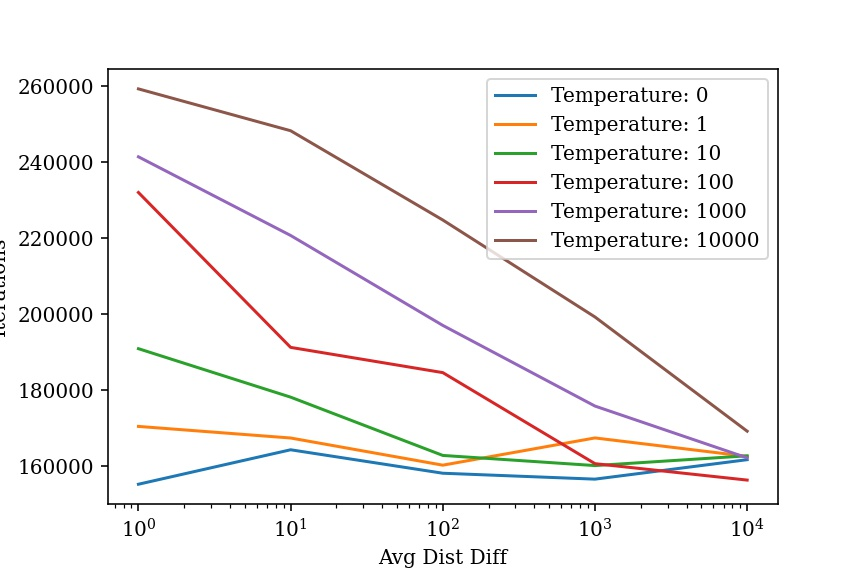
\includegraphics[width=1\linewidth]{images/rand_temperature_avg_dist_diff_iterations.jpg}
        \caption{Optimality for each cooling rate}
        \label{fig:sub2}
    \end{subfigure}
    \captionsetup{justification=centering}
    \caption{Absolute comparison between final distances, and iterations, for different $T_0$}
\end{figure}


\begin{figure}[H]
    \centering
    \begin{subfigure}{0.45\textwidth}
        \centering
        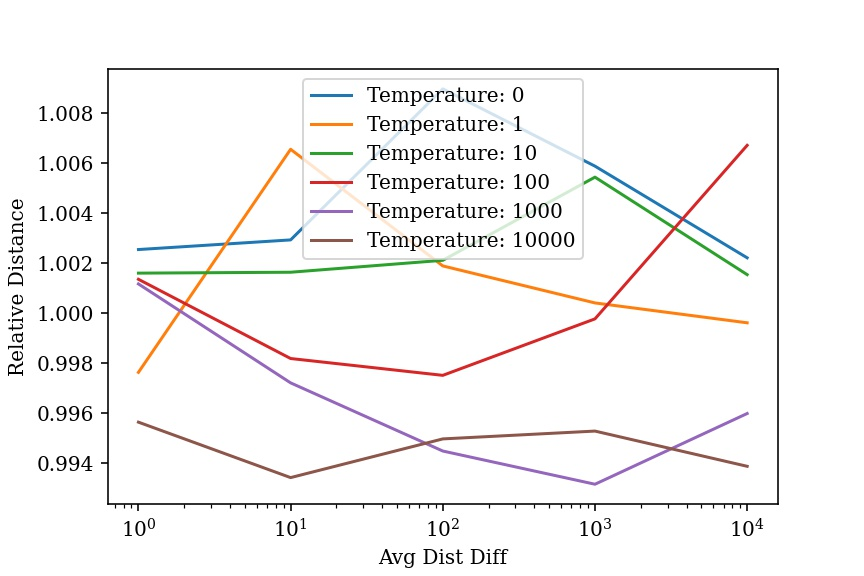
\includegraphics[width=1\linewidth]{images/rand_temperature_avg_dist_diff_distance_relative.jpg}
        \caption{Final distance for different }
        \label{fig:sub1}
    \end{subfigure}%
    \begin{subfigure}{0.45\textwidth}
        \centering
        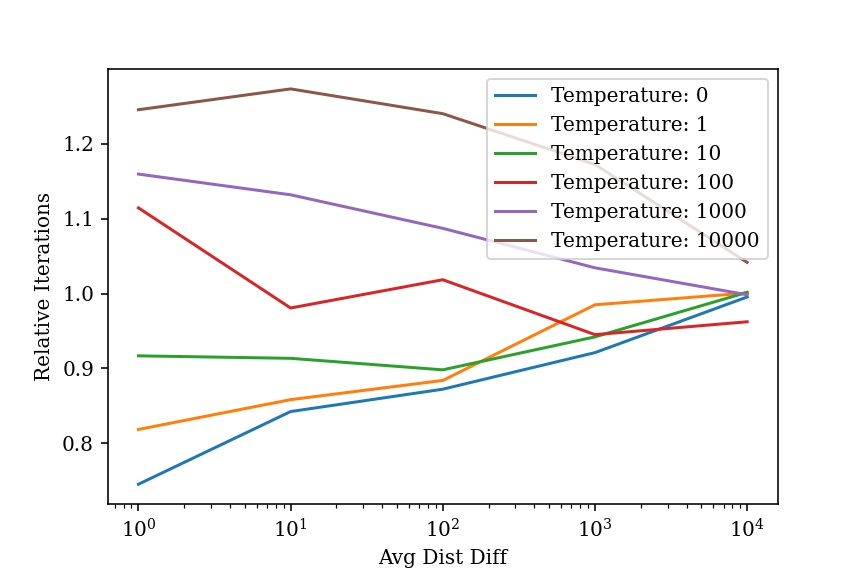
\includegraphics[width=1\linewidth]{images/rand_temperature_avg_dist_diff_iterations_relative.jpg}
        \caption{Optimality for each cooling rate}
        \label{fig:sub2}
    \end{subfigure}
    \captionsetup{justification=centering}
    \caption{Relative comparison between final distances, and iterations, for different $T_0$}
\end{figure}

\subsubsection{Discussion}

\textbf{Cooling Rate}
\\

There was a clear trend between a slower cooling rate and a greater relative optimality, and this effect seemed to increase the greater the city count.
Note $r$ is the cooling rate and $n$ is the number of cities.

\begin{figure}[H]
    \centering
    \begin{tabular}{ |c|c|c|c|c|c|c| } 
        \hline
        & \thead{$n = 10^1$} & \thead{$n \approx 10^{1.5}$} & \thead{$n = 10^2$} & \thead{$n \approx 10^{2.5}$} & \thead{$n = 10^{3}$} & \thead{$n \approx 10^{3.5}$} \\
        \hline
        $r = 0$       & 1.000 & 1.000 & 1.000 & 1.000 & 1.000 & 1.000 \\
        \hline
        $r = 0.9$     & 1.027 & 1.304 & 1.989 & 2.619 & 2.946 & 3.052 \\
        \hline
        $r = 0.99$    & 1.038 & 1.323 & 2.339 & 4.024 & 6.480 & 8.574 \\
        \hline
        $r = 0.999$   & 1.041 & 1.360 & 2.338 & 4.263 & 8.213 & 14.74 \\
        \hline
        $r = 0.9999$  & 1.044 & 1.406 & 2.411 & 4.292 & 8.374 & 16.12 \\
        \hline
        $r = 0.99999$ & 1.044 & 1.415 & 2.525 & 4.443 & 8.391 & 16.21 \\
        \hline
    \end{tabular}
    \caption{Table comparison between cooling rate and iterations}
\end{figure}

\begin{figure}[H]
    \centering
    \begin{subfigure}{0.5\textwidth}
        \centering
        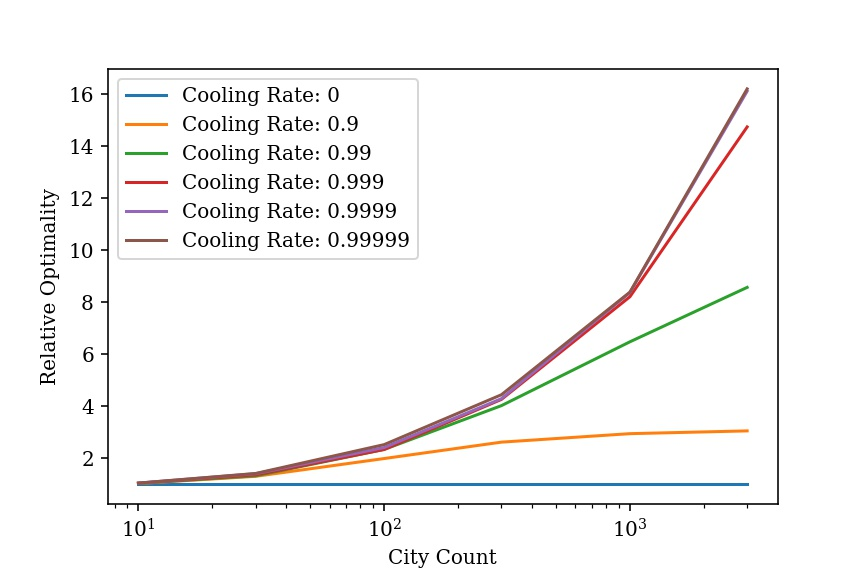
\includegraphics[width=1\linewidth]{images/rand_cooling_rate_city_count_distance_relative-to-base.jpg}
    \end{subfigure}%
    \begin{subfigure}{0.5\textwidth}
        \centering
        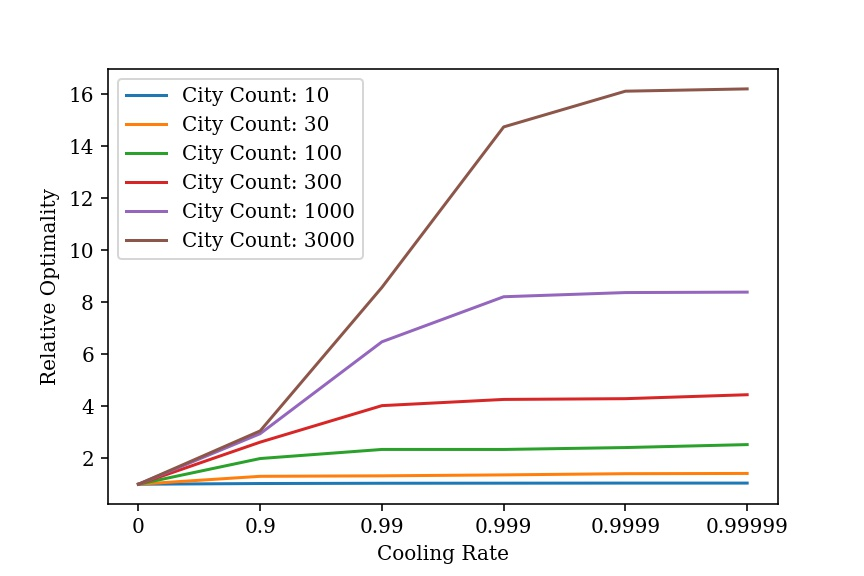
\includegraphics[width=1\linewidth]{images/rand_cooling_rate_city_count_distance_relative-to-base-transpose.jpg}
    \end{subfigure}
    \captionsetup{justification=centering}
    \caption{Plot comparison between cooling rate and iterations}
\end{figure}

Overall, having a slower cooling rate allowed us to find a more optimal solution.
This increase in optimality would be even more pronounced for greater city counts - as it was likely that a greedy solution on average would get stuck in a local minimum.
\\

However, there seemed to be a limit of how much better a Simulated Annealing solution could be compared to a greedy method, and this limit would be proportional to the city count.
\\

Overall this trend follows that of a logistic curve, where if we take $r' = -\log_{10}(1 - r)$, i.e. if $r = 0.9$, then $r' = 1$, if $r = 0.99$, then $r' = 2$, and so on, the relative optimality could be determined by the function

$$f(r', n) = \frac{L}{1 + e^{-k(r'-r'_0)}}$$

\begin{figure}[H]
    \centering
    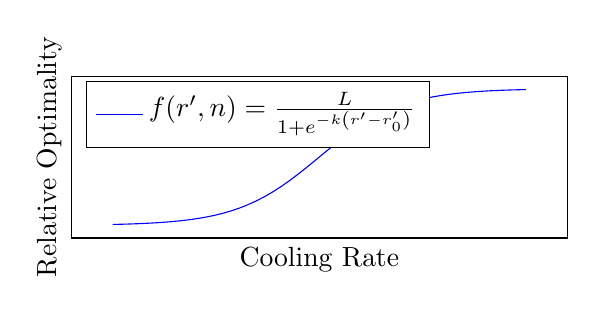
\begin{tikzpicture}
        \begin{axis}[
            width=0.65\textwidth,
            height=0.3\textwidth,
            xlabel=Cooling Rate,
            ylabel={Relative Optimality},
            xtick=\empty,
            ytick=\empty,
            legend pos=north west
        ]
        \addplot[
            blue,
            mark=none,
            samples=50,
            domain=0:2000
        ]
        (x,{10/(1+exp(-0.005 * (x - 1000)))});
        \addlegendentry[text depth=0.7em]{$f(r', n) = \frac{L}{1 + e^{-k\left(r' - r_0'\right)}}$}
        \end{axis}
    \end{tikzpicture}
    \caption{Example of a logistic curve}
\end{figure}

where

\begin{itemize}
    \item $L$ is the curve's maximum value. \\
    Whilst this is an unreachable asymptote, it's value for a city count above 30 can be predicted to be
    $$L \approx 0.45 + 4^{\log_{10}(n) - 1.5}$$
    
    \item $r_0'$ is the $r'$ value of the sigmoid point. \\
    As a result, $r_0' = r_1' / 2$ if at cooling rate $r_1'$ we reach close to the highest possible optimality (or the asymptote), and so is around
    $$r_0' \approx \log_{10}(n) - 1$$
    
    \item $k$ is the logistic growth rate or steepness of the curve. \\
    We need to ensure that at a cooling rate of 0 will result in a relative optimality of 1, i.e. $f(r = 0, n) = 1$ and hence
    
    $$1 = \frac{L}{1 + e^{-k(r' - r_0')}} \approx \frac{0.45 + 4^{\log_{10}(n) - 1.5}}{1 + e^{-k(-\log_{10}(n) - 1)}}.$$
    
    Therefore, 
    \begin{align*}
        1 + e^{-k(-\log_{10}(n) - 1)}
            &\approx 0.45 + 4^{\log_{10}(n) - 1.5} \\
        -k(-\log_{10}(n) - 1)
            &\approx \ln(4^{\log_{10}(n) - 1.5} - 0.55) \\
        k
            &\approx \frac{\ln(4^{\log_{10}(n) - 1.5} - 0.55)}{\log_{10}(n) - 1}.
    \end{align*}
\end{itemize}

This can be pieced together to form a prediction of the relative optimality based off the cooling rate and city count.
\\

More importantly though, this can be used to determine the point at which a slower cooling rate results in a lesser increase in optimality. 
Whilst the inflection point of the curve can be used (which is also $r'_0$), it tends to be around half of the optimal value that can be achieved.
Another value that can be used is finding the value of $r'$ that produces the lowest value in the second derivative (this value also represents the value of the "maximal growth period").
\\

That being said, these calculations are highly dependent on the experimental results and resulted in very convoluted equations.
Something more suitable may have been an approximation that produces around $80 - 90\%$ of the optimal solution.
This value tended can be determined as
$$r \approx 1 - 100^{-log_{10}(n)+1}.$$


% DERIVATIVE STUFF WHICH DEPENDED TOO HARD ON EXPERIMENT VALUES
% As shown in the graph below, it correlates to around $80 - 90\%$ of the maximal optimal value that can be achieved.

% \begin{align*}
%     f &= \frac{L}{1 + e^{-k(r' - r'_0)}} \\
%     \frac{\partial f}{\partial r} &= -\frac{Lke^{-k\left(-r'+r'_0\right)}}{\left(1+e^{-k\left(r'_0-r'\right)}\right)^2} \\
%     \frac{\partial^2 f}{\partial r^2} &= -\frac{Lk^2e^{-2k\left(r'_0-r'\right)}\left(e^{k\left(r'_0-r'\right)}-1\right)}{\left(1+e^{-k\left(r'_0-r'\right)}\right)^3} \\
% \end{align*}


% \begin{figure}[H]
%     \centering
%     \begin{tikzpicture}
%         \begin{axis}[
%             width=1\textwidth,
%             height=0.4\textwidth,
%             xtick=\empty,
%             ytick={0},
%             legend pos=north west,
%             ymajorgrids=true,
%             grid style=dashed
%         ]
%         % \draw (1.5,0) -- (1.5,1);
%         \addplot[
%             black,
%             mark=none,
%             samples=100,
%         ]
%         (x, {1/(1+exp(-x)))});
%         \addlegendentry{$f$}
%         \addplot[
%             gray,
%             mark=none,
%             samples=100,
%         ]
%         (x, {
%             1 * (1/(1+exp(-x))))*(1-(1/(1+exp(-x)))))
%         });
%         \addlegendentry{$\frac{\partial f}{\partial r'}$}
%         \addplot[
%             blue,
%             mark=none,
%             samples=100,
%         ]
%         (x, {
%             10 * exp(-2 * x) * (-exp(x)+1) / ((1+exp(-x))^3)
%         });
%         \addlegendentry{$\frac{\partial^2 f}{\partial r'^2}$}
%         % \draw[dotted] (axis cs:\pgfkeysvalueof{/pgfplots/xmin},0) -- (axis cs:\pgfkeysvalueof{/pgfplots/xmax},0);
%         \end{axis}
%     \end{tikzpicture}
% \end{figure}

% Finding the value of $r$ that produces the lowest value of $\frac{\partial^2 f}{\partial r^2}$ is the larger value of which the third derivative is equal to 0.
% This can be calculated by substituted our determined values of $L, k, r'_0$ into the equation

% $$
%     \frac{\partial^3 f}{\partial r'^3}
%     = -\frac{
%         Lk^3e^{-3k\left(r'_0-r'\right)}\left(e^{2k\left(r'_0-r'\right)}-4e^{k\left(r'_0-r'\right)}+1\right)
%     }{
%         \left(1+e^{-k\left(r'_0-r'\right)}\right)^4
%     }
%     = 0.
% $$

% This can be simplified to finding

% \begin{align*}
%     e^{2k\left(r'_0-r'\right)} - 4e^{k\left(r'_0-r'\right)}+1 &= 0 \\
%     \ln(2k\left(r'_0-r'\right)) &= 4\ln(k\left(r'_0-r'\right)) \\
%     2k\left(r'_0-r'\right) &= (k\left(r'_0-r'\right))^4 \\
%     \frac{2}{k^3} &= (r'_0 - r')^3 \\
%     \frac{\sqrt[3]{2}}{k} &= (r'_0 - r')
% \end{align*}


The number of iterations increased linearly with the city count where,
$$\text{if } r = 0, \: \text{iterations} \approx 10n.$$

There was a clear trend between a slower cooling rate and an increase in the number of iterations.

This is because with a slower cooling rate, the temperature remains higher for longer.
For example, if the starting temperature was $T_0$, the following number of iterations are required to reach a portion of the initial temperature.

\begin{figure}[h]
    \centering
    \begin{tabular}{ |c|c|c| } 
        \hline
        \thead{Cooling Rate} & \thead{Iterations to \\reach $0.1T_0$} & \thead{Iterations to \\ reach $0.01T_0$} \\ 
        \hline
        0.9     & 22     & 44 \\
        \hline
        0.99    & 230    & 459 \\
        \hline
        0.999   & 2302   & 4603 \\ 
        \hline
        0.9999  & 23025  & 46050 \\
        \hline
        0.99999 & 230258 & 460515 \\
        \hline
    \end{tabular}
    \caption{Number of iterations required to lower the temperature by a certain percent}
\end{figure}


\begin{figure}[H]
    \centering
    \begin{subfigure}{0.45\textwidth}
        \begin{tabular}{ |c|c|c| } 
            \hline
            \thead{Cooling Rate} & \thead{Relative \\ Iterations} & \thead{Increase \\ from prev.} \\
            \hline
            0       & 1   & N/A  \\
            \hline
            0.9     & 6   & 6    \\
            \hline
            0.99    & 27  & 4.5  \\
            \hline
            0.999   & 80  & 2.96 \\
            \hline
            0.9999  & 180 & 2.25 \\
            \hline
            0.99999 & 516 & 2.87 \\
            \hline
        \end{tabular}
    \end{subfigure}%
    \begin{subfigure}{0.55\textwidth}
        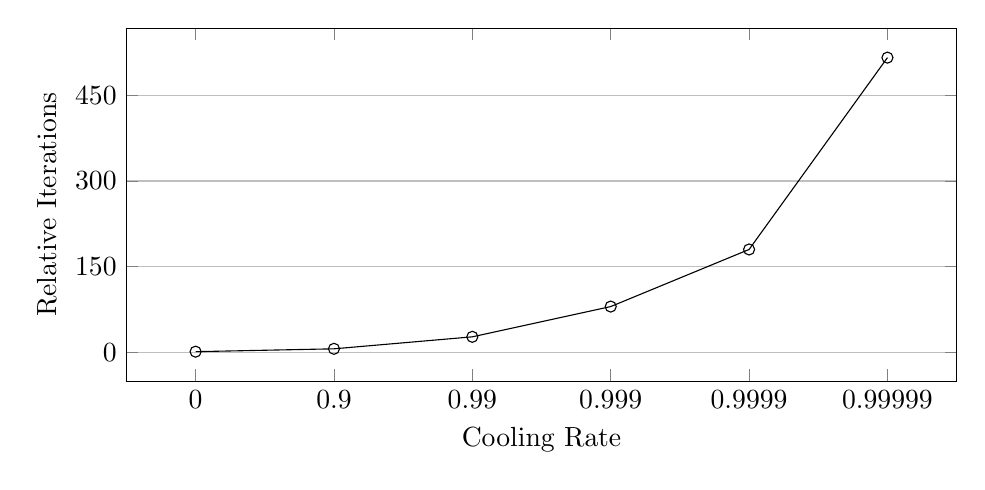
\begin{tikzpicture}
            \begin{axis}[
                height=0.5\textwidth,
                width=1\textwidth,
                xlabel={Cooling Rate},
                ylabel={Relative Iterations},
                xtick={0, 1, 2, 3, 4, 5},
                xticklabels={0, 0.9, 0.99, 0.999, 0.9999, 0.99999},
                ytick={0, 150, 300, 450},
                ymajorgrids=true,
            ]
            \addplot[mark=o]
                coordinates {
                (0,1)(1,6)(2,27)(3,80)(4,180)(5,516)
                };
            \end{axis}
        \end{tikzpicture}
    \end{subfigure}
    \captionsetup{justification=centering}
    \caption{Raw comparison between cooling rate and iterations from experiments}
\end{figure}

Whilst there aren't enough points to verify, if the relative iterations grow polynomially or exponentially, it can be determined that the increase in iterations scales faster than the optimality.
\\

Hence, at least for cooling rates in the range $0 - 0.99999$, you do not receive a greater increase in optimality relative to the increase in iterations from slowing the cooling rate.
\\

Interestingly, the relative increase in iterations from the experimental results for each cooling rate are lower than those required for the temperature to reach a certain percentage of it's initial temperature.
This suggests that the solution starts to converge before at different temperatures for different cooling rates.
\\

\newpage
\textbf{Temperature}

Relative optimality in the final distance by changing the temperature was mostly negligible compared to changing the cooling rate.
However, each $T_0$ typically produced it's best final distance, if it was equal to the average difference in distances between the cities. 
Higher temperatures also tended to provide better results, however they also resulted in a greater number of iterations.
\\

\begin{figure}[H]
    \centering
    \begin{tabular}{ |c|c|c|c|c|c| } 
        \hline
        & \thead{$\Delta d = 10^0$} & \thead{$\Delta d = 10^1$} & \thead{$\Delta d = 10^2$} & \thead{$\Delta d = 10^3$} & \thead{$\Delta d =  10^4$} \\
        \hline
        $T_0 = 0$     & 1.0026 & 1.0029 & 1.0090 & 1.0059 & 1.0022 \\
        \hline
        $T_0 = 10^{0}$ & 0.9976 & 1.0066 & 1.0019 & 1.0004 & 0.9996 \\
        \hline
        $T_0 = 10^{1}$ & 1.0016 & 1.0016 & 1.0021 & 1.0054 & 1.0016 \\
        \hline
        $T_0 = 10^{2}$ & 1.0014 & 0.9982 & 0.9975 & 0.9998 & 1.0067 \\
        \hline
        $T_0 = 10^{3}$ & 1.0012 & 0.9972 & 0.9945 & 0.9932 & 0.9960 \\
        \hline
        $T_0 = 10^{4}$ & 0.9957 & 0.9934 & 0.9950 & 0.9953 & 0.9939 \\
        \hline

    \end{tabular}
    \caption{Table comparison between relative final distance and temperature}
\end{figure}

Overall, a better conclusion may have been determined if there were more tests, though there is already previous research to suggest that a value of $T_0$ relative to the average loss is ideal \cite{initial-temperature}.
\\

Interestingly, if the temperature was very high relative to the average difference in distance between the cities, it underwent a lot of iterations.
However, as the average distance between cities increased, the number of iterations decreased, despite the number of cities remaining the same.
\\

This is because when the temperature is too high, a worse configuration is more or less always accepted.
As a result, it does not converge to a solution.

% Absolute final distance
% [42, 418, 4213, 42085, 419304]
% [42, 420, 4184, 41856, 418217]
% [42, 418, 4185, 42066, 419023]
% [42, 416, 4165, 41829, 421186]
% [42, 416, 4153, 41553, 416699]
% [41, 414, 4155, 41642, 415816]


% Absolute iterations
% [155246, 164317, 158142, 156586, 161710]
% [170466, 167416, 160263, 167435, 162576]
% [190929, 178171, 162828, 160157, 162728]
% [232048, 191272, 184628, 160661, 156337]
% [241440, 220734, 197058, 175823, 162193]
% [259319, 248302, 224802, 199270, 169206]

% Relative final distance
% [1.0026, 1.0029, 1.0090, 1.0059, 1.0022]
% [0.9976, 1.0066, 1.0019, 1.0004, 0.9996]
% [1.0016, 1.0016, 1.0021, 1.0054, 1.0016]
% [1.0014, 0.9982, 0.9975, 0.9998, 1.0067]
% [1.0012, 0.9972, 0.9945, 0.9932, 0.9960]
% [0.9957, 0.9934, 0.9950, 0.9953, 0.9939]


% Relative iterations
% [0.7455, 0.8425, 0.8723, 0.9212, 0.9954]
% [0.8186, 0.8584, 0.8840, 0.9850, 1.0007]
% [0.9169, 0.9135, 0.8982, 0.9422, 1.0017]
% [1.1143, 0.9807, 1.0184, 0.9451, 0.9623]
% [1.1594, 1.1318, 1.087-, 1.0343, 0.9984]
% [1.2453, 1.2731, 1.2400, 1.1723, 1.0415]

\\


%%%%%%%%%%%%%%%%%%%%%%%%%%%%%%%%%%%%%%%%%%%%%%%%%%%%%%%%%%%%%%%%%%%%%%%%%%%%%%%%
%%%%%%%%%%%%%%%%%%%%%%%%%%%%%%%%%%%%%%%%%%%%%%%%%%%%%%%%%%%%%%%%%%%%%%%%%%%%%%%%
\newpage
\section{Conclusion}
Whilst there are faster and more optimal algorithms for TSP, we noted that the cooling rate could be parameterised off the number of cities, and the temperature by the average distance between the cities.
\\

Overall the cooling rate had a much bigger impact than the temperature on both the final distance found, and the number of iterations.
Slower cooling rates and higher initial temperatures often resulted in lower final distances, however also resulted in high iterations and hence solving time.
\\

Whilst slower cooling rates resulted in better solutions, there was a limit of how much better it could be relative to the greedy solution.
Hence, there was a point at which slowing the cooling rate more resulted in a negligible increase in optimality.
Whilst not experimented with, this is likely also the case with increasing the temperature, however, there is little purpose for doing so as there is comparatively small benefit from increasing the temperature.
\\

A suitable value of the cooling rate that provided around $90\%$ of the most optimal solution could be calculated as 
$$r \approx 1 - 100^{-\log_{10}(n) + 1}.$$

A suitable value of the temperature was one that was proportional to the average difference in distance of the cities.
This could be calculated in $O(n\log n)$ using a sliding window approach in the following pseudo code:

\begin{verbatim}
from math import dist

def get_diff_city_dist(cities: list[tuple[int, int]]) -> float:
    n = len(cities)
    d = sorted([dist(cities[i], cities[j]) for i in range(n-1) for j in range(i+1,n)])
    m = len(d)
    
    prev_diff = sum([x - d[0] for x in d[1:]])
    total_diff = prev_diff
    for i in range(1, m):
        prev_diff = prev_diff - (d[i] - d[i - 1]) * (m - i)
        total_diff += prev_diff
    
    return total_diff / ((m * (m - 1)) / 2)
\end{verbatim}

Unfortunately the runtime was not tested the experimentation as it may have been sensitive to the testing environment.
However, it would be interesting to see the runtime relative to the rest of the parameters, as may not scale exactly with iterations.
This is because the runtime of an iteration would be $O(n)$ if it accepts a new configuration, else $O(1)$.
As a result, this would also give insight into details such as how the probability of accepting a different configuration changes with temperature, and the current optimality of the solution.


%%%%%%%%%%%%%%%%%%%%%%%%%%%%%%%%%%%%%%%%%%%%%%%%%%%%%%%%%%%%%%%%%%%%%%%%%%%%%%%%
%%%%%%%%%%%%%%%%%%%%%%%%%%%%%%%%%%%%%%%%%%%%%%%%%%%%%%%%%%%%%%%%%%%%%%%%%%%%%%%%
\newpage
\section{References}
\bibliographystyle{standard}
\begin{thebibliography}{9}

\bibitem{cook12}
Cook, William J. (2012). \emph{In Pursuit of the Traveling Salesman: Mathematics at the Limit of Computation.} Princeton, NJ: Princeton UP

\bibitem{helsgaun98}
K. Helsgaun, (1998). \emph{An Effective Implementation of the Lin-Kernighan Traveling Salesman Heuristic. DATALOGISKE SKRIFTER (Writings on Computer Science), No. 81} Roskilde University.

\bibitem{metropolis}
N.A. Metropolis, A. Rosenbluth, M. Rosenbluth, A. Teller, and E. Teller. (1953) \emph{Equation of state calculations by
fast computing machines} J. Chem. Phys, vol. 21, pp. 1087–1092

\bibitem{kirkpatrick}
S. Kirkpatrick, C.D. Gelatt, and M.P. Vecchi, “Optimization by simulated annealing,” Science, vol. 220, pp.
671–680, 1983

\bibitem{tsplib}
G. Reinelt, (1991). \emph{TSPLIB - A Traveling Salesman Problem Library”,} ORSA J. Comput., 3-4, 376-385.

\bibitem{cooling-schedule}
Mahdi, Walid \& Medjahed, Seyyid Ahmed \& Ouali, Mohammed. (2017). \emph{Performance Analysis of Simulated Annealing Cooling Schedules in the Context of Dense Image Matching.} Computación y Sistemas. 21. 493-501.

\bibitem{fixed-temperature}
Fielding, M. (2000). \emph{Simulated Annealing With An Optimal Fixed Temperature.} SIAM J. Optim., 11, 289-307.

\bibitem{initial-temperature}
Ben-Ameur, Walid. (2004). \emph{Computing the Initial Temperature of Simulated Annealing. Computational Optimization and Applications.} 29. 369-385.



\end{thebibliography}

\end{document}
